% !TeX program = pdflatex
% FluxPhased — Task-level adversarial co-adaptation of radar and jammer teams
% Target venue: IEEE Transactions on Aerospace and Electronic Systems (TAES)
\documentclass[journal]{IEEEtran}

\usepackage{amsmath,amssymb,amsfonts}
\usepackage{graphicx}
\usepackage{booktabs}
\usepackage{multirow}
\usepackage{xcolor}
\usepackage{cite}
\usepackage[hidelinks]{hyperref}
\usepackage{url}
% paper/math_commands.tex
\newcommand{\E}{\mathbb{E}}
\newcommand{\R}{\mathbb{R}}
\newcommand{\etaN}{\eta}
\newcommand{\dropRatio}{d}
\newcommand{\snr}{\mathrm{SNR}}
\newcommand{\jnr}{\mathrm{JNR}}
\newcommand{\hth}{\mathrm{h2h}}
\newcommand{\jvs}{\mathrm{jvs}}
\newcommand{\jone}{\mathrm{j1}}
\newcommand{\radidle}{\mathrm{rad\mbox{-}idle}}


\title{Scaling the Attack Breaks Defense Containment in Task-Level Radar--Jammer Self-Play}
\author{Anonymous Authors}

\begin{document}
\maketitle
\begin{abstract}
Modern multifunction phased-array radars must schedule heterogeneous missions while facing coordinated, adaptive interference. Link-level signal-to-interference ratios do not by themselves reveal whether a radar network completes its deadline-constrained mission load. We introduce FluxPhased, a physics-grounded task-level benchmark for adversarial co-adaptation between multifunction radars and cooperative jammers. Missions carry service and bearing identities, deadlines, and exact detection credit; the link model combines generalized planar-array responses with finite jammer energy budgets. A pre-training contestability test and a four-view evaluation protocol separate natural scheduling loss from adversarial loss.

In a one-jammer versus two-radar game, the valid 12-dB S6 runs neutralize $63.7\%\pm1.0\%$ of the jammer's floor-adjusted disruptive power across two training seeds. When the attacker team is doubled under the same 63-token team budget, three converged seeds yield a stable 2v2 equilibrium with head-to-head mission drop $0.3366\pm0.0143$ and neutralization $23.0\%\pm1.1\%$. Radar competence against idle jammers remains low, showing that the degradation is an offensive scaling effect rather than a corresponding defender collapse. A co-located-jammer control attributes most of the change to attacker count under the S7 separated-radar geometry (neutralization $28.4\%$), with cross-fire geometry contributing a further reduction to $24.2\%$. Finally, a lightweight opponent-class mixture reduces singleton relative leverage from $0.502$ to $0.262$ at 75\% singleton exposure, with the largest neutralization value at 50\% exposure. The results establish a measurable separation between equilibrium stability, attack scaling, and opponent-distribution robustness.

\end{abstract}

\begin{IEEEkeywords}
Radar resource management, multifunction radar, phased arrays, electronic warfare, electronic attack, mission scheduling, multi-agent reinforcement learning, self-play, adversarial robustness.
\end{IEEEkeywords}

\section{Introduction}
Electronic-support and electronic-attack systems interact through a resource-constrained loop: an interferer chooses where and when to spend energy, while a multifunction radar chooses which service and bearing to observe before each mission deadline. A high instantaneous JNR can be operationally irrelevant if the radar detects the corresponding target in another dwell, whereas a modest interference pulse can matter when it arrives at the only vulnerable point in a deadline window. The operational outcome is therefore mission completion, not a single link-budget scalar.

This distinction exposes a gap between two established lines of work. Radar--jammer learning studies formulate waveform, frequency, or power decisions as sequential games. Multifunction-radar scheduling studies optimize scan and track allocation under time or power constraints. These lines of work leave open a system-level question: how does the balance of an adaptive game change when the number of coordinated attackers increases while the defender's mission workload and total interference budget remain fixed?

We answer this question with a controlled S6-to-S7 progression in FluxPhased. S6 contains one learned jammer and two learned radar heads. S7 contains two parameter-shared jammer agents and two parameter-shared radar agents. The S7 team receives a 63-cell activation budget, split 32/31 between jammers. This controls total jammer activation while the radar-site geometry changes from S6 to S7; the matched co-located-jammer control isolates the additional cross-fire component within the S7 geometry.

The main result is a change in containment, not a corresponding failure of learning. Across three S7 seeds trained to 3000 iterations, head-to-head mission drop is $0.3366\pm0.0143$, compared with $0.0860\pm0.0061$ in the valid three-seed 12-dB S6 baseline. The floor-adjusted fraction of marginal jammer disruption removed by learned radars falls from $62.8\%\pm1.6\%$ to $23.0\%\pm1.1\%$. The radar floor against idle jammers remains low ($0.0194\pm0.0008$ in S7 versus $0.0242\pm0.0097$ in valid S6), and the S7 trajectory is stationary from approximately iteration 1700 through 3000. Thus, the second attacker changes the stable equilibrium's scale while preserving low idle-jammer loss and training stability.

Evaluation-only scripted baselines bound these equilibrium numbers. Both learned teams clearly beat random and fixed-stare scripted opponents, but a greedy mission-stare radar holds mission drop at $0.0889$ against every trained jammer team---below the learned head-to-head value and below the natural scheduling floor. The head-to-head drop is therefore an equilibrium property of the co-adapted pair, not a ceiling on radar performance, and both teams are specialized to their training opponents.

This paper makes five contributions:
\begin{enumerate}
    \item We formulate a test-and-evaluation protocol for learned radar resource management under adaptive electronic attack, coupling deadline-constrained mission loss to array-factor link physics, finite energy, and two-team multi-agent PPO. Its three components---the pre-training contestability gate, the floor-adjusted containment metric $\eta$, and the evaluation-only scripted anchors---are each independently reusable test instruments, separable from the specific learner used here.
    \item We quantify a benchmark-level attacker-count scaling effect: with total jammer activation controlled, doubling attackers reduces the mission-denial containment of learned radar scheduling by roughly two-thirds, with replication across three converged S7 seeds, a three-seed valid S6 reference, and a three-seed co-located control.
    \item We use a matched co-located-jammer control to decompose the mechanism under the separated S7 radar geometry. Two jammers already reduce containment to $26.6\%\pm2.9\%$ across three control seeds; cross-fire adds a secondary reduction to $24.2\%$.
    \item We anchor both learned teams with evaluation-only scripted baselines. Both teams dominate random and stare policies, but a greedy mission-stare radar is unexploited by every trained jammer team, showing that head-to-head drop is an equilibrium quantity rather than a radar performance ceiling.
    \item We test a minimal opponent-class mixture. The singleton-to-pair disruption ratio falls from $0.502$ to $0.262$ as singleton exposure increases, identifying opponent-class mixing as a practical robustness intervention while documenting its training-budget confound.
\end{enumerate}

The rest of the paper defines the benchmark and evaluation metric, presents convergence and scaling results, tests the count--geometry decomposition, analyzes opponent-specific adaptation, and evaluates the lightweight mixing intervention. We use ``drop'' for the fraction of eligible missions that are not completed before their deadlines; higher drop therefore indicates greater jammer-side success.

\section{Related Work}
\subsection{Learning in radar--jammer games}
Recent radar anti-jamming studies have used multi-agent reinforcement learning and game-theoretic formulations to adapt waveform, frequency, and power decisions. Neural fictitious self-play (NFSP) has been applied to imperfect-information games, and related radar studies use game-based learning for frequency-agile and waveform decisions. These studies establish adaptive radar--jammer interaction as a useful game formulation, but their principal outcomes are link-level quantities such as SINR, detection probability, or waveform utility. FluxPhased complements this line with a mission-level endpoint: a target is successful only when the appropriate service detects the appropriate bearing within a deadline window \cite{heinrich2016deep}.

\subsection{Multifunction-radar resource management}
A separate literature treats multifunction-radar scheduling as an MDP or constrained MDP. Deep Q-learning, actor--critic methods, PPO, SAC, and model-based planning have been applied to scan--track allocation, congested task scheduling, and time or power budgeting. These approaches address the central scheduling trade-off that a radar cannot attend to every task at every instant. They generally use fixed or scripted interference conditions, however, and therefore do not measure how a learning radar changes when the adversary co-adapts. Our benchmark retains the scheduling structure of this literature while adding a learning jammer team and an explicit natural-floor control.

\subsection{Self-play, specialization, and leagues}
Self-play can produce strong coordination but can also specialize agents to the distribution of partners or opponents encountered during training \cite{heinrich2016deep,vinyals2019alphastar,wang2020roma}. Role-oriented multi-agent learning relates team performance to emergent division of labor, and population-based training addresses opponent diversity rather than a single opponent trajectory. The hierarchical macro-strategy model for MOBA games likewise separates high-level target allocation from low-level execution and uses cross-agent coordination \cite{wu2018moba}. We borrow these ideas as motivation; R5 tests a minimal opponent-class mixture, not a full population-based league.

\subsection{Position of this work}
FluxPhased lies at the intersection of these communities. Its agents learn link-facing actions, but the reported endpoint is task completion under service, bearing, deadline, and energy constraints. This enables a controlled question that link-level or single-sided scheduling studies do not answer: whether an apparent defensive advantage survives attacker-count scaling. The resulting comparison is designed around three controls: the idle-radar floor, a scripted-radar jammer view, and a co-located-jammer ablation. The controls let us separate absolute loss, adversarial marginal loss, equilibrium stability, and robustness to a changed opponent class.

\section{Benchmark and Method}
\subsection{Task-level mission model}
At each time step, each service can receive an arrival. An admitted mission is represented by
\begin{equation}
 m=(s,a,t_{\mathrm{arr}},t_{\mathrm{dl}},n_{\mathrm{det}}),
\end{equation}
where $s$ is the service, $a\in\{0,\ldots,4\}$ is its azimuth sector, and the deadline is at most six steps after arrival. A mission succeeds when the radar team obtains one detection with the exact $(s,a)$ identity before the deadline. The tracker credits the oldest incomplete mission with the matching service and bearing; detections at the deadline are processed before finalization. The mission drop ratio counts timeouts, admission rejects, and horizon failures over eligible missions:
\begin{equation}
 \dropRatio=\frac{N_{\mathrm{to}}+N_{\mathrm{rej}}+N_{\mathrm{hz}}}{N_{\mathrm{elig}}}.
\end{equation}
A larger value means that the jammer team denied more missions. We retain completed-but-not-yet-finalized missions in the queue, which makes the deadline accounting explicit and auditable.

\subsection{Bearing-aware link physics}
Each agent selects a beam from a $5\times5$ azimuth--elevation grid. A jammer selects a Bernoulli mask over 25 array cells and a categorical beam. For a steering direction $(u_b,v_b)$ and target $(u_t,v_t)$, the normalized planar-array response is separable and follows the standard uniform-planar-array power pattern for a $5\times5$ element grid:
\begin{align}
 G_{\mathrm{AF}}(b,t)=\;&10\log_{10}\!\left(\frac{A_{5}(u_t-u_b)^2}{5^2}\right)\nonumber\\
 &+10\log_{10}\!\left(\frac{A_{5}(v_t-v_b)^2}{5^2}\right),
\end{align}
where $A_5$ is the finite-array element factor response evaluated with the same float32 implementation for all experiments; the separable form is the usual product of azimuth and elevation linear-array factors \cite{skolnik2008,vantrees2002}. For jammer $k$ and radar $r$, the received JNR includes jammer cell aggregation, transmit and receive array gains at their pair bearing, service-dependent path loss and receiver gain, and polarization loss. Independent jammers are combined as incoherent power:
\begin{equation}
 \label{eq:jnrsum}
 \jnr_r=10\log_{10}\sum_k10^{\jnr_{kr}/10}.
\end{equation}
The effective SNR is
\begin{equation}
 \snr_{\mathrm{eff},r}=10\log_{10}\left(\frac{10^{\snr_0/10}}{1+10^{\jnr_r/10}}\right)+G_{\mathrm{coh}},
\end{equation}
with the idle case defined by $\jnr_r=-\infty$. A mission at azimuth $a$ is detected with
\begin{equation}
 p_{r}(s,a)=\sigma\left(\frac{\snr_{\mathrm{eff},r}+G_{\mathrm{target}}(b_r,a)-\tau}{w}\right),
\end{equation}
where $\tau=15$ dB and $w=3$ dB. This couples radar pointing to both useful detection gain and exposure to interference.

Table~\ref{tab:linkbudget} lists the complete link-budget parameterization. The per-pair received JNR follows the standard one-way interference budget $\jnr_{kr}=P_{\mathrm{tx}}+G_{\mathrm{tx}}+G_{\mathrm{rx}}-L_{\mathrm{path}}-L_{\mathrm{pol}}+10\log_{10}(\text{spectral overlap})-N$ with free-space path loss $L_{\mathrm{path}}=20\log_{10}(4\pi d/\lambda)$ and noise $N=-174+10\log_{10}B+\mathrm{NF}$~\cite{neri2006book}; it omits atmospheric and rain terms, which are small at X-band over 8~km relative to the dB-scale margins studied here.

\begin{table}[t]
\caption{Link-budget and detection parameters.}
\label{tab:linkbudget}
\centering
\footnotesize
\setlength{\tabcolsep}{4pt}
\begin{tabular}{ll}
\toprule
Parameter & Value \\
\midrule
Service 0 & $f_c=10.0$ GHz, $B=10$ MHz, $G_{\mathrm{rx}}=35$ dB \\
Service 1 & $f_c=10.5$ GHz, $B=20$ MHz, $G_{\mathrm{rx}}=30$ dB \\
Jammer power per cell & $P_{\mathrm{jam}}=0.1$ W \\
Jammer Tx gain & 20 dB \\
Jammer--radar range & $d=8$ km (floor 100 m) \\
Polarization loss & 3 dB \\
Noise figure & 5 dB \\
Coherent gain & $G_{\mathrm{coh}}=20$ dB \\
Baseline SNR & $\snr_0=12$ dB \\
Threshold / width & $\tau=15$ dB, $w=3$ dB \\
\bottomrule
\end{tabular}
\end{table}

Two combining assumptions deserve justification. First, \emph{within} one jammer, active cells are aggregated with phase-aligned contributions, i.e., the cell mask acts as idealized transmit beamforming; this isolates the scheduling question (which cells, which beam) from array calibration error. Second, \emph{across} jammers, received powers are summed incoherently in~(\ref{eq:jnrsum}). The two jammer sites are separated by a baseline of approximately $2d\sin 60^\circ\approx13.9$~km, i.e., about $5\times10^5$ wavelengths at 10~GHz; without phase coordination at that scale, the received phase difference is uniformly uncertain, so expected received powers---not fields---add. Coherent cross-jammer combining would require phase synchronization far beyond the threat model assumed here and would only strengthen the attacker; the incoherent model is therefore the conservative choice for the defense-side conclusions. The jamming waveform is broadband noise with rectangular spectra, so service-dependent rejection enters only through the spectral-overlap factor; we do not model pulse-to-pulse agility, Doppler, or MTI filtering, and Section~VII discusses this boundary.

\subsection{S6 and S7 games}
S6 uses one jammer against two co-located learned radar heads. S7 uses two parameter-shared jammers at azimuths $+60^\circ$ and $-60^\circ$ and two radar heads at $+20^\circ$ and $-20^\circ$. Both stages use the validated $\snr_0=12$ dB regime and $P_{\mathrm{jam}}=0.1$ W per active cell. The S7 team receives a total 63-token budget, split 32/31 between jammers; the S6-to-S7 comparison therefore changes attacker count and radar-site geometry while holding total S7 jammer activation fixed.

Each side uses a parameter-shared multi-head actor. Radar agents choose beam and service; jammer agents choose cell mask and beam. Table~\ref{tab:spaces} summarizes the action and observation spaces. A centralized privileged critic receives the concatenated public observations of its team during training, while the deployable actor receives only its local observation and last-action ESM channels. PPO uses generalized advantage estimation, clipped likelihood ratios, per-head entropy schedules, and separate actor, local critic, and privileged-critic optimizers \cite{yu2022surprising,schulman2017proximal}. Rollouts flatten agent slots in agent-major order so the shared team reward is duplicated without mixing trajectories.

\begin{table}[t]
\caption{Action and observation spaces.}
\label{tab:spaces}
\centering
\footnotesize
\begin{tabular}{lll}
\toprule
 & Jammer agent & Radar head \\
\midrule
Actions & cell mask (25 Bern.) & beam (25-way) \\
 & beam (25-way) & service (2-way) \\
Energy & 32/31-token budget & unconstrained \\
Obs.\ dim & 67 & 60 \\
Obs. & own energy, & pending $(s,a)$ map, \\
 & radar beams/svcs/ & own+partner beams \\
 & detected flags, & and services, \\
 & pending map, & per-jammer DOA \\
 & partner channel & and active flags \\
Privileged & team cat.\ (134) & team cat.\ (120) \\
\bottomrule
\end{tabular}
\end{table}

\subsection{Evaluation and containment}
We evaluate four views for S7: head-to-head (h2h), learned jammers against scripted sweep radars (jvs), learned radars against idle jammers (rad-idle), and one learned jammer against the pair-trained radars (j1-only). The S6 baseline defines h2h, jvs, rad-idle, and the natural floor; it does not contain the S7-specific j1-only control. The scripted sweep against idle jammers supplies the natural floor $d_{\mathrm{floor}}$. Let $d_{\mathrm{h2h}}$, $d_{\mathrm{jvs}}$, and $d_{\mathrm{idle}}$ denote the corresponding drop ratios.
\begin{equation}
 \eta=1-\frac{d_{\mathrm{h2h}}-d_{\mathrm{idle}}}{d_{\mathrm{jvs}}-d_{\mathrm{floor}}}.
\end{equation}
This metric measures the fraction of the jammer's marginal disruption that learning radars remove; it avoids crediting the radar for losses caused by its own scheduling floor. Three properties matter for interpretation. $\eta=1$ when the learned radars push the head-to-head drop back to their own idle-jammer drop; $\eta=0$ when the marginal adversarial loss equals the full scripted-radar exposure, i.e., the learned radar removes none of it; values between 0 and 1 are directly readable as removed fractions. The denominator $d_{\mathrm{jvs}}-d_{\mathrm{floor}}$ is the game's realizable disruption range, so $\eta$ is comparable across games only when that range is similar---we therefore always report it alongside the raw drops. Finally, $\eta$ is an equilibrium quantity: it measures containment by the co-adapted radar policy, not the best achievable containment against a frozen opponent (Section~V-C). Final evaluations use 64 fixed validation scenarios and three independent action seeds (4242, 777, and 31337).

\subsection{Pre-training contestability gate}
Before training, we enumerate beam responses for each mission azimuth. The gate requires at least three of five azimuths to have best-response detection probability in $(0.05,0.95)$, a minimum above 0.02, and a maximum above 0.8. The S7 cross-fire profile is $(0.837,0.912,0.989,0.993,0.855)$; all five sectors remain reachable and three remain contestable. The co-located-jammer control profile is $(0.921,0.823,0.989,0.996,0.991)$, which predicts a more defense-favorable game before any policy update.

\begin{figure*}[t]
\centering
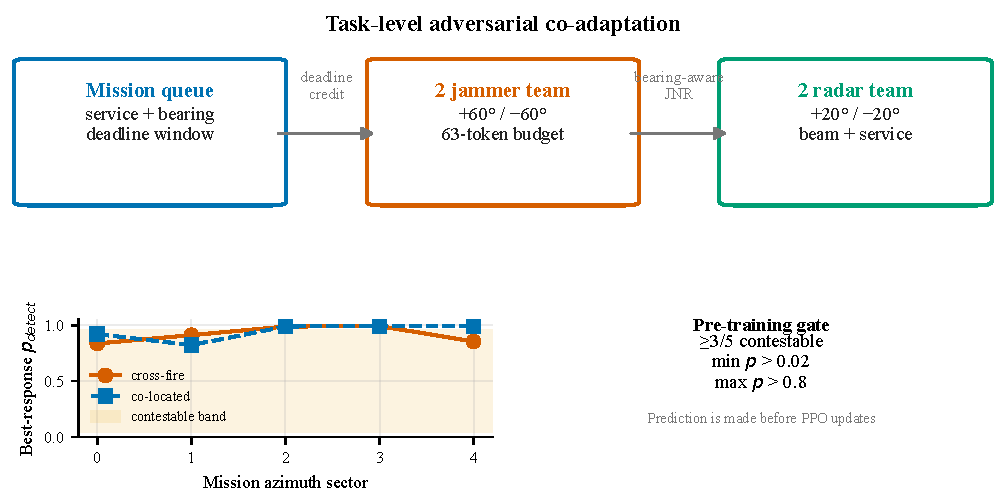
\includegraphics[width=0.96\textwidth]{figures/fig1_benchmark_anatomy.pdf}
\caption{Benchmark anatomy and pre-training contestability. FluxPhased couples a deadline-constrained mission queue to bearing-aware jammer--radar link physics. The lower panel reports the best-response detection profiles used to gate the cross-fire and co-located configurations before training.}
\label{fig:benchmark}
\end{figure*}

\section{Experimental Protocol}
\subsection{Training and checkpoints}
We use 64 fixed training scenarios and a separate 64-scenario validation manifest. Each environment rollout has 16 parallel environments and a 64-step horizon. The S7 main experiments use three random seeds (20260801, 20260802, and 20260803). Each seed trains for 1000 iterations with the normal per-head entropy schedule and continues to 3000 iterations with entropy coefficients frozen at their minimum. The continuation isolates additional optimization from a second exploration schedule. Table~\ref{tab:hyper} lists the shared training configuration.

\begin{table}[t]
\caption{Training hyperparameters (both teams, both stages).}
\label{tab:hyper}
\centering
\footnotesize
\setlength{\tabcolsep}{4pt}
\begin{tabular}{ll}
\toprule
Parameter & Value \\
\midrule
Environments $\times$ horizon & $16\times64$ \\
Actor / critic LR & $3\times10^{-5}$ / $10^{-3}$ \\
Discount $\gamma$ / GAE $\lambda$ & 0.99 / 0.95 \\
PPO clip / grad clip & 0.2 / 0.5 \\
Epochs / minibatch & 4 / 256 \\
Target KL (rollback) & 0.02 \\
Entropy coef.\ (cell, beam, svc) & $2{\times}10^{-2}$, $5{\times}10^{-3}$, $10^{-2}$ \\
Entropy anneal frac.\ (c,b,s) & 0.7, 0.9, 0.5 \\
Priv.\ value / distill coef. & 0.5 / 0.1 \\
Value loss coef. & 0.5 \\
Iterations (stage 1 / 2) & 1000 / 2000 (frozen) \\
\bottomrule
\end{tabular}
\end{table}

The primary S6 comparison uses the three valid 12-dB training seeds 20260730, 20260731, and 20260732. An earlier S6 seed, 20260729, was trained accidentally with a 22-dB override; we exclude it from the primary comparison and retain it only as a documented regime check. The valid three-seed S6 aggregate is used wherever an S6 uncertainty is reported.

The co-located-jammer control uses the same 1000+1000 two-stage protocol, the same 63-token team budget, radar sites at $+20^\circ$ and $-20^\circ$, and both jammer sites at $+60^\circ$, replicated across three training seeds (20260811--20260813); its evaluation passes the explicit \texttt{+60,+60} geometry to the evaluator. (An initial single-seed evaluation of seed 20260811 was first generated with the default cross-fire geometry; that file is retained as an audit artifact and no reported number uses it.)

\subsection{Algorithm and counter-adaptation controls}
Two controls isolate what the results do and do not attribute to the learning rule and to the training opponent distribution. The IPPO control trains four independent PPO learners (per-agent actors and local critics, no parameter sharing, no centralized critic) in the same game under the same two-stage protocol; everything except the learning rule is bit-identical, so it tests whether the containment collapse is specific to MAPPO. The counter-adaptation control inverts the training: the radar side is pinned to the greedy mission-stare heuristic (its update is skipped), and only the jammer team learns, for 2000 iterations. Its validation metric is the greedy radar's drop against the evolving jammer team, compared with the $0.0889$ static baseline.

\subsection{Opponent-class mixture}
R5-lite trains one seed for each singleton exposure fraction $q\in\{0.25,0.50,0.75\}$, for 2000 iterations under the same two-stage protocol. On a fraction $q$ of iterations, jammer 1 is forced idle and the radar team updates against the singleton opponent; the jammer-team update is skipped on those iterations. This is a minimal opponent-class mixture rather than a full population league. The reference $q=0$ is the S7 seed-01 2000-iteration checkpoint. Because jammer updates are skipped on singleton iterations, the absolute jammer strength changes with $q$. We therefore treat $j1/jvs$, $h2h/jvs$, and $\eta$ as the primary cross-condition readouts and present absolute drops as descriptive context.

\subsection{Statistical reporting}
For S7, the final evaluation runs four views over all 64 validation scenarios with one repetition for each of three action seeds. The S6 implementation supplies h2h, jvs, rad-idle, and the natural floor but does not supply the S7-specific j1-only control. We report the mean and standard deviation across action seeds for each training seed. Aggregate S7 values report the mean and standard deviation across the three training seeds. The natural floor is computed using scripted radar sweeps against idle jammers under the same environment regime. We retain all raw JSONL logs and final evaluation JSON files in the repository artifact tree.

\subsection{Evaluation-only scripted baselines}
Each converged checkpoint is additionally evaluated against five scripted baselines that require no training. The random radar samples beam and service uniformly from the legal sets; the greedy mission-stare radar points each head at the pending service--azimuth cell with the most missions, read from the radar observation; the earliest-deadline-first (EDF) radar points each head at the pending mission with the earliest deadline---unlike the others this is an oracle heuristic, because deadline state is not part of the radar observation; the random jammer activates one uniformly random legal cell and beam per step while energy remains; the stare jammer holds the horizon-plane beam closest to its paired radar-site bearing with one active cell until the budget is spent. Stare beam indices are computed from the site geometry rather than tuned. These views use the same 64 validation scenarios and three action seeds, so they are directly comparable with the learned views. They anchor both teams against non-learning behavior and expose whether the self-play policies are specialized to their training opponents.

\subsection{Implementation checks}
The S7 environment and physics tests contain 18 contract and physics gates. They cover action shapes, energy accounting, exact service--bearing credit, generalized array-factor consistency, two-source JNR summation, detection monotonicity, observation channels, ledger identity, and pre-training contestability. Atomic checkpoints and a max-iteration resume criterion protect long runs from interrupted sessions. These engineering checks are separate from the scientific result and are reported to make the training trajectory reproducible.

\section{Results}
\subsection{Self-play converges to stable task-level equilibria}
The first question is whether mission-level self-play produces a reproducible endpoint rather than a transient training phase. Figure~\ref{fig:training} shows the full three-stage trajectory for S7 seed 20260801.
\begin{figure}[t]
\centering
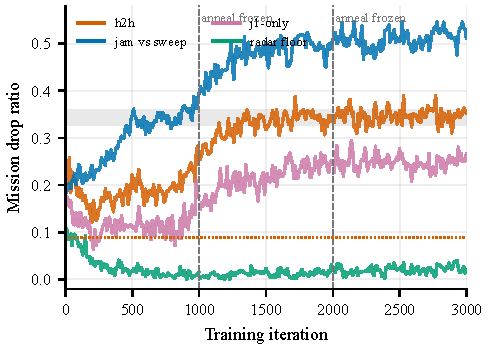
\includegraphics[width=\columnwidth]{figures/fig2_training_curves.pdf}
\caption{Three-stage S7 trajectory for seed 20260801. Dashed lines mark the 1000- and 2000-iteration continuation boundaries; the final region is stationary across the four evaluation views.}
\label{fig:training}
\end{figure} After the entropy schedule was frozen, the five 200-iteration windows from 2000 to 3000 had h2h means 0.3465, 0.3428, 0.3484, 0.3507, and 0.3463. The corresponding jam-vs-sweep means were 0.5121, 0.4956, 0.5118, 0.5107, and 0.5215. This continuation therefore rules out both an early stopping artifact and a persistent drift. The last 40 validation points at 3000 give h2h $0.3485\pm0.0151$ and jam-vs-sweep $0.5161\pm0.0174$.

The same endpoint appears across three converged S7 seeds. Full-protocol evaluation gives h2h drops of 0.3390, 0.3212, and 0.3496, with an across-seed mean of $0.3366\pm0.0143$. The idle-radar drop is $0.0194\pm0.0008$ in S7, compared with $0.0242\pm0.0097$ across the three valid S6 seeds; both values remain low. The convergence result is descriptive: it establishes a stable attractor for this benchmark and training protocol, not a proof of global Nash equilibrium.

A response-set exploitability measure sharpens what stationarity does and does not imply. We evaluate each team against every alternative response in our evaluation set and sum the best deviation gains, an upper-bound-free, response-set-restricted analog of NashConv. The jammer team has no improving deviation in the set: the trained pair's drop of $0.3366$ exceeds the singleton ($0.2086\pm0.0745$), the stare pair ($0.2374\pm0.0036$), and the random pair ($0.0922\pm0.0047$) against the same radars. The radar team does: deviating to the greedy mission-stare policy recovers $0.3366-0.0889=0.2477$ of drop against the same jammers. The response-set exploitability of the converged pair is therefore $0.2477$, driven entirely by the radar side. We report this as a lower bound over an enumerated response set, not exact exploitability: it quantifies that the stationarity of Fig.~\ref{fig:training} reflects mutual co-adaptation within the training distribution, while a measurable exploit remains available to out-of-distribution responses---the phenomenon that Sections~V-C and V-D develop.

The containment result also survives a change of learning rule. An IPPO control---four independent PPO learners, no parameter sharing, no centralized critic, everything else bit-identical---reaches the same 2000-iteration protocol point at h2h $0.2472$, jam-vs-sweep $0.4123$, and neutralization $23.3\%$, versus $0.3282$, $0.5043$, and $20.2\%$ for MAPPO at the same budget. Absolute levels differ on both sides, but the floor-adjusted containment ratio barely moves: the attacker-count effect is a property of the game's structure, not of MAPPO's centralized critic, and $\eta$ itself is robust to the learner's strength.

\subsection{Doubling the attacker reduces defense containment by two-thirds}
The main comparison is summarized in Table~\ref{tab:main} and Figure~\ref{fig:neutralization}.
\begin{figure}[t]
\centering
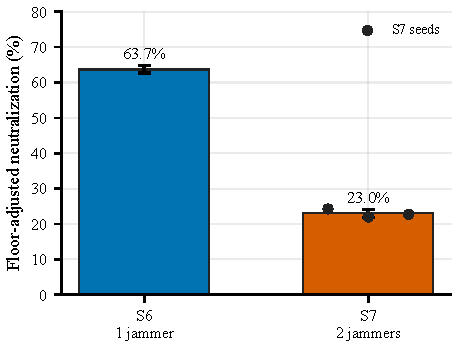
\includegraphics[width=\columnwidth]{figures/fig3_neutralization.pdf}
\caption{Floor-adjusted neutralization for the S6 and S7 games. The dots show the three converged S7 training seeds; error bars are standard deviations across training seeds (S6 uses the three valid 12-dB seeds).}
\label{fig:neutralization}
\end{figure} In S6, the valid three-seed 12-dB h2h drop is $0.0860\pm0.0061$, jam-vs-sweep is $0.2727\pm0.0088$, and floor-adjusted neutralization is $62.8\%\pm1.6\%$. In converged S7, these values become $0.3366\pm0.0143$, $0.5294\pm0.0215$, and $23.0\%\pm1.1\%$, respectively.

The neutralization change is not a consequence of a corresponding radar collapse. Learned radars facing idle jammers retain a low drop of $0.0194\pm0.0008$ in S7, compared with $0.0242\pm0.0097$ across the three valid S6 seeds. Instead, two jammers increase the marginal disruption that survives radar adaptation. The jammer team's raw disruption against scripted sweeps rises by 94\% relative to S6, while the fraction of that disruption removed by learned radars falls by approximately two-thirds. Because the comparison controls total jammer activation but also changes radar-site geometry, this is a benchmark-level scaling result rather than a fully isolated attacker-count intervention.

\begin{table}[t]
\caption{Converged S6--S7 comparison. Drop is the mission-loss ratio; $\eta$ is floor-adjusted defense neutralization.}
\label{tab:main}
\centering
\small
\begin{tabular}{lcc}
\toprule
Metric & S6: 1v2 & S7: 2v2 \\
\midrule
h2h drop & $0.0860\pm0.0061$ & $0.3366\pm0.0143$ \\
jam-vs-sweep drop & $0.2727\pm0.0088$ & $0.5294\pm0.0215$ \\
rad-vs-idle drop & $0.0242\pm0.0097$ & $0.0194\pm0.0008$ \\
$\eta$ & $62.8\%\pm1.6\%$ & $23.0\%\pm1.1\%$ \\
\bottomrule
\end{tabular}
\end{table}

\subsection{Scripted baselines anchor both teams and expose co-adaptation}
Table~\ref{tab:baselines} evaluates the converged teams against four scripted policies under the identical 64-scenario, three-action-seed protocol. Both learned teams dominate their non-learning counterparts: a random legal radar loses $0.5085\pm0.0051$ of missions against the trained jammer pairs versus $0.3366\pm0.0143$ for the trained radar team, and random or stare jammers impose only $0.0922\pm0.0047$ and $0.2374\pm0.0036$ against the trained radars versus $0.3366\pm0.0143$ for the trained jammer pairs. Learning is real on both sides of the link.

\begin{table}[t]
\caption{Evaluation-only scripted baselines against the converged S7 teams (mission drop; mean $\pm$ sd across three training seeds, three action seeds each). EDF is a deadline-informed oracle (privileged deadline state).}
\label{tab:baselines}
\centering
\small
\begin{tabular}{lc}
\toprule
Policy & Mission drop \\
\midrule
\multicolumn{2}{l}{\emph{Radar side, vs.\ trained jammer pairs}} \\
Learned radar team (h2h) & $0.3366\pm0.0143$ \\
Scripted sweep & $0.5294\pm0.0215$ \\
Random legal radar & $0.5085\pm0.0051$ \\
Greedy mission-stare radar & $0.0889\pm0.0000$ \\
EDF oracle radar & $0.2961\pm0.0039$ \\
\midrule
\multicolumn{2}{l}{\emph{Jammer side, vs.\ trained radar teams}} \\
Learned jammer pair (h2h) & $0.3366\pm0.0143$ \\
Stare jammer pair & $0.2374\pm0.0036$ \\
Random legal jammer pair & $0.0922\pm0.0047$ \\
Idle jammers (reference) & $0.0194\pm0.0008$ \\
\bottomrule
\end{tabular}
\end{table}

The greedy mission-stare radar is the informative exception. Pointing both heads at the heaviest pending service--azimuth cell yields a drop of exactly $0.0889$ against every trained jammer pair and every action seed---a factor of 3.8 below the learned h2h drop and below even the natural scheduling floor of $0.1187$ (sweep radars facing idle jammers). The zero variance is not an evaluation artifact: the greedy policy is deterministic given the observations, and none of the jammer action streams sampled across nine (team, action-seed) combinations flips any per-step detection outcome under the stare margin, so mission completion is fully determined by the arrival and scheduling process. (Its three-decimal coincidence with the S6 h2h value 0.0888 is chance; the two numbers come from independent evaluation pipelines over different games.) Under this link budget, the pointing gain at the exact mission bearing creates a detection margin that none of the three trained jammer teams overcomes: their learned advantage applies to radars that spread attention (sweeps, $0.5294$; the learned equilibrium radar, $0.3366$), not to a well-pointed stare. The ordering among heuristics is itself diagnostic: the hottest-queue stare ($0.0889$) dominates a deadline-first oracle ($0.2961\pm0.0039$) despite the latter's privileged deadline access, because per-step detection is probabilistic and grinding the densest pending sector converts more expected detections than chasing the single earliest deadline.

This reframes the h2h value and $\eta$: they are equilibrium quantities, not radar performance ceilings. The self-play radar hedges against its co-trained opponent at the cost of mission throughput, and the learned jammer team is exploitable by an out-of-distribution non-learning policy---the radar-side counterpart of the singleton result in Section~V-D. A jammer team co-trained against greedy radars would plausibly restore the penalty; testing that counter-adaptation requires new training runs and is left as future work.

\subsection{When does pointing discipline dominate?}
The stare result can be decomposed analytically. Holding the jammer allocation fixed and varying only the radar beam, exact mission-bearing pointing weakly dominates the neighboring beam at \emph{every} azimuth and \emph{every} jammer power we tested (0.1--12.8 W per cell): the pointing-gain term always exceeds the exposure penalty, so per-step detection satisfies $p_{\mathrm{exact}}\ge p_{\mathrm{off}}$ by construction of the link budget. Within a deadline window of at most six steps, the success probabilities compound as $1-(1-p)^{6}$, so even a factor-of-two per-step advantage compounds into an overwhelming window advantage. Pointing discipline is therefore always weakly optimal per target; the residual scheduling question is \emph{which} mission to point at when several contend, which is where the heuristic ordering of Table~\ref{tab:baselines} comes from. The hottest-queue rule concentrates both heads on the densest pending sector, converting each step into two independent detection trials on the same mission; the EDF oracle instead chases the single earliest deadline, spreading the same looks across sectors and paying the off-bearing pointing loss on most of them. Under stochastic per-step detection, concentrating looks on the densest sector maximizes expected completions per step, which is why the oracle's privileged deadline knowledge buys less than queue density.

The absolute survival level, however, is strategic rather than physical. We recomputed the stare window success under a worst-case aimed jammer pair (both jammers choosing the received-power-maximizing beam against the stared radar, one cell each, the deployed per-step activation): the six-step success probability collapses to between 0.004 and 0.317 depending on azimuth, versus near-unity under the fixed benign allocation used in the pre-training gate (Fig.~\ref{fig:benchmark}). The trained jammer teams play mixed beam policies between these two bounds, and the observed greedy-stare success of $0.911$ lies in that interval. A budget-concentration scan sharpens the boundary: stacking 2 cells in a single aimed step already reduces the worst-azimuth stare window success below $10^{-3}$. The stare margin that the trained teams leave on the table is thus a property of their learned allocation, not of the physics---precisely the question the counter-adaptation control (jammers trained against a fixed stare radar) is designed to answer.

\subsection{Attacker count is primary; cross-fire geometry is secondary}
The co-located-jammer control tests whether the S7 result requires two spatially separated jammers. It places both jammer sites at $+60^\circ$ while retaining the two radar sites at $\pm20^\circ$, the same physics, budget, two-stage training, and final evaluation, replicated across three training seeds. The control yields h2h $0.3033\pm0.0102$, jam-vs-sweep $0.4978\pm0.0081$, and neutralization $26.6\%\pm2.9\%$ (per-seed $28.4\%$, $23.2\%$, $28.1\%$).

Thus, the matched S7 geometry control shows that two jammers account for most of the containment loss within the separated-radar setting: containment is $26.6\%\pm2.9\%$ for co-located jammers and $24.2\%$ for cross-fire. The S6-to-S7 comparison additionally changes radar-site geometry, so the full count effect is a benchmark-level attribution rather than a perfectly isolated causal contrast. The cross-fire comparison itself is controlled for radar placement, budget, training protocol, and evaluation. The pre-specified contestability profiles and the matched control are shown in Figure~\ref{fig:benchmark}; the converged mechanism decomposition is shown in Figure~\ref{fig:ablation}.
\begin{figure*}[t]
\centering
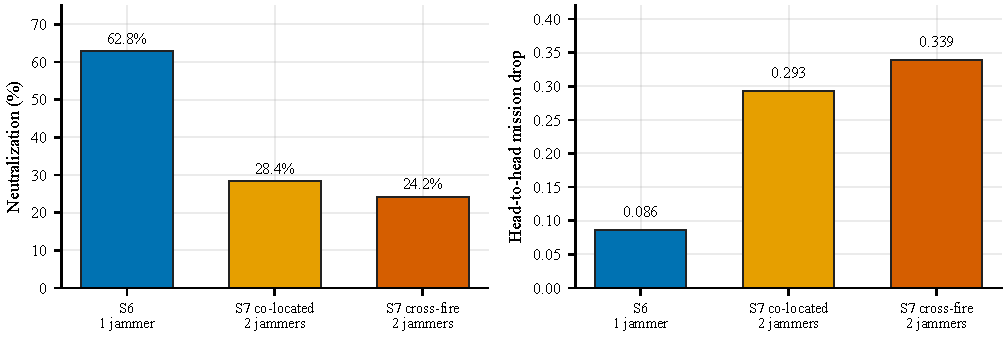
\includegraphics[width=0.96\textwidth]{figures/fig4_mechanism_ablation.pdf}
\caption{Mechanism decomposition under matched task, budget, and training protocols. Two co-located jammers reproduce most of the containment loss, while cross-fire geometry adds a secondary penalty.}
\label{fig:ablation}
\end{figure*}

\subsection{Containment saturates beyond two attackers at fixed budget}
The attacker-count axis extends beyond the matched control by training the n-jammer game at $n=3$ (sites $+60^\circ, 0^\circ, -60^\circ$, budget split 21/21/21) under the identical two-stage protocol, with the $n=2$ cross-fire run as the reference. Pre-training gate profiles computed with the exact published semantics reproduce the $n=2$ profile digit-for-digit and pass for the arc placement, so the extension stayed inside the validated regime. Across three converged $n=3$ seeds, neutralization is $22.2\%\pm1.5\%$ (h2h $0.224$, jam-vs-sweep $0.362$)---statistically indistinguishable from the $n=2$ value of $24.2\%$, while the raw disruption against scripted sweeps \emph{falls} from $0.529$ to $0.362$.

The scaling picture is therefore not monotone in attacker count at fixed total budget: the containment break occurs at the $1\to2$ step ($62.8\%$ to mid-20s), and adding a third jammer neither deepens it nor further erodes containment. The per-jammer budget, not the count, becomes the binding variable---21 tokens per jammer dilute each site's peak disruptive power below what the pairwise equilibrium extracts from 31--32 tokens. For defense design this is the useful direction of the result: the stress test that matters is the transition from one source to two, and beyond that the antagonist's total energy budget dominates its distribution across platforms.

\subsection{Counter-adaptation: the stare margin is learnable to attack}
The greedy-stare result of Section~V-C leaves open whether a jammer team \emph{could} punish the stare or merely had not. The counter-adaptation control answers it: training the jammer team against a fixed greedy-stare radar (radar updates skipped) drives the stare's drop from the static $0.0889$ to $0.213$ by iteration 2000---a factor of 2.4, still trending upward at the end of the run. Three consequences follow. The zero-variance baseline was not an evaluation artifact: a co-trained opponent moves it. The margin is strategic rather than physical, exactly as the worst-case-aimed analysis of Section~V-C predicted (the aimed bound sits at $0.68$--$1.00$ drop). And plain self-play simply never visited the stare in its opponent distribution---the same specialization failure that Section~V-D exposed on the radar side, now demonstrated on the jammer side under training.

\subsection{Pair-trained defenses trade singleton robustness for pairwise defense}
The fourth view evaluates one learned jammer against radars trained in the 2v2 game. Across the three converged S7 seeds, the singleton drop is 0.2632, 0.2387, and 0.1238, with mean $0.2086\pm0.0745$. This variation is larger than the h2h variation, but all three seeds expose the same opponent-class boundary: a defense optimized against a pair is not uniformly robust to a singleton. The spread itself is mechanistically plausible---the pair-trained radar heads divide the azimuth plane between sectors, and how well that division happens to cover the surviving jammer's bearing varies per seed---and the per-seed behavior extractions in the artifact allow this attribution to be checked directly.

The seed-01 continuation makes the trade-off visible over time. As the pair-trained equilibrium develops, j1-only rises from approximately 0.12 near the 1000-iteration checkpoint to approximately 0.24 at 2000 and remains near 0.25 at 3000, while h2h settles near 0.34. Radar competence against idle jammers remains low and stable. The result is therefore an adaptation trade-off, not evidence that the radar actor or critic stopped learning.

The learned behavior is interpretable and is summarized in Figure~\ref{fig:behavior}.
\begin{figure*}[t]
\centering
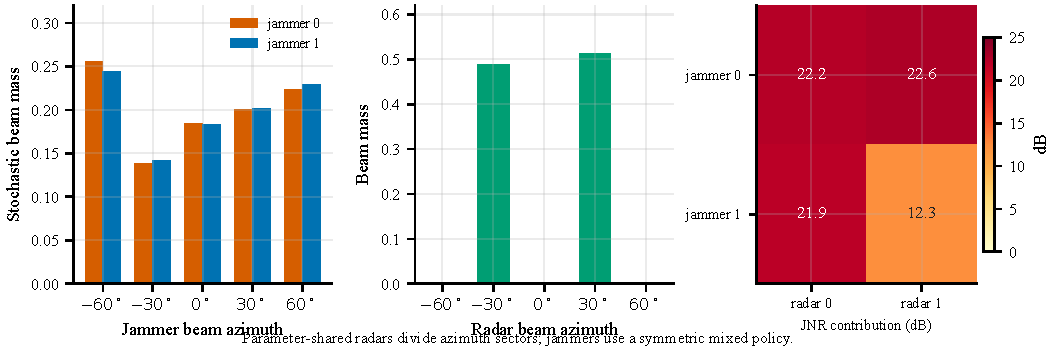
\includegraphics[width=0.96\textwidth]{figures/fig5_behavior.pdf}
\caption{Equilibrium behavior at the converged S7 checkpoint. Radar heads divide the mission plane between two azimuth sectors, while the jammer team uses a symmetric mixed beam policy. The heat map reports active-only pairwise JNR contributions in dB.}
\label{fig:behavior}
\end{figure*}

\subsection{Opponent-class mixing reduces singleton leverage}
The full dose-response is shown in Figure~\ref{fig:r5} and Table~\ref{tab:r5}.
\begin{figure}[t]
\centering
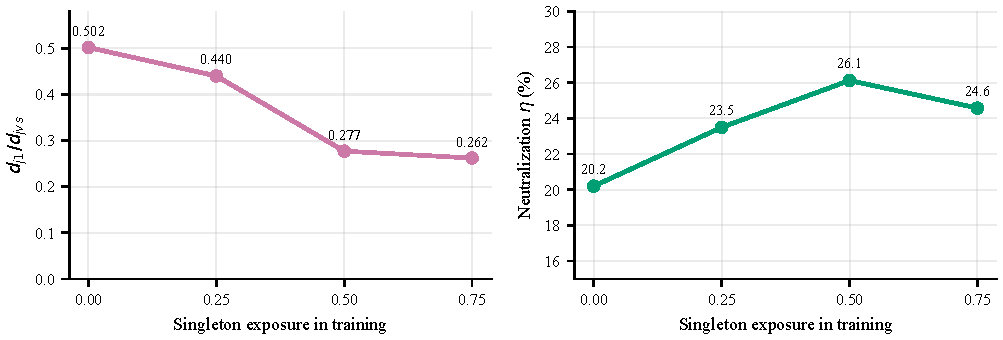
\includegraphics[width=\columnwidth]{figures/fig6_r5_dose_response.pdf}
\caption{R5-lite opponent-class mixing. Singleton relative leverage $d_{j1}/d_{jvs}$ falls with singleton exposure, while floor-adjusted neutralization peaks near 50\%. Absolute drops are confounded by skipped jammer updates.}
\label{fig:r5}
\end{figure}
\begin{table}[t]
\caption{R5-lite opponent-class mixture. Absolute drops are descriptive because singleton iterations skip the jammer update; ratio metrics are the primary comparison.}
\label{tab:r5}
\centering
\small
\begin{tabular}{lccccc}
\toprule
$q$ & h2h & jvs & j1-only & j1/jvs & $\eta$ \\
\midrule
0 & .3282 & .5043 & .2532 & .502 & 20.2\% \\
.25 & .2470 & .4015 & .1767 & .440 & 23.5\% \\
.50 & .1962 & .3580 & .0992 & .277 & 26.1\% \\
.75 & .1939 & .3476 & .0911 & .262 & 24.6\% \\
\bottomrule
\end{tabular}
\end{table}

Singleton relative leverage $d_{\mathrm{j1}}/d_{\mathrm{jvs}}$ falls monotonically from 0.502 to 0.262 and saturates between 50\% and 75\% exposure. The containment ratio $\eta$ increases from 20.2\% to 26.1\% at 50\% exposure before leveling at 24.6\%. The h2h-to-jvs ratio is $0.651$ at $q=0$, falls to $0.548$ at $q=0.50$, and is $0.558$ at $q=0.75$. It therefore improves through the 50\% condition and changes little thereafter; the ratio-level data do not show a pairwise-versus-singleton trade-off in this intervention.

R5-lite has an important design boundary. On singleton iterations, jammer 1 is forced idle and its update is skipped; consequently the jammer team receives fewer gradient updates as $q$ increases, and absolute jvs drops from 0.5043 to 0.3476. The dose-response does not identify a causal improvement in absolute radar performance. It does support a narrower intervention claim: under this minimal mixture and fixed training budget, exposing the radar team to a singleton opponent reduces the singleton's relative leverage, with diminishing returns after 50\% exposure. A gradient-aligned multi-seed experiment is needed before calling the result universal.

\section{Discussion}
The experiments reveal a distinction that is hidden by link-level reporting. Increasing the attacker team from one to two does not make self-play unstable; it changes how much of the jammer's marginal disruption the learned radar team can remove. Under the tested task workload, the same radar competence floor coexists with a much larger adversarial loss. The relevant design variable is therefore not only the quality of a single radar policy, but also the number and spatial arrangement of simultaneous interference sources.

The scripted baselines add a second distinction: an equilibrium policy is not a mission-optimal policy. The learned jammer teams cannot punish a greedy mission-stare radar (drop $0.0889$, invariant across all three trained teams), while they punish sweeps ($0.5294$) and the learned radar ($0.3366$). Both sides of the self-play game are specialized to the training opponent distribution: the radar gives up mission throughput to hedge against its co-trained jammer, and the jammer's disruption is effective precisely against attention-spreading radars. Head-to-head drop and containment $\eta$ must therefore be read as properties of the co-adapted pair, not as absolute radar or jammer ratings. This is the same lesson as the singleton-vulnerability result, seen from the other side of the game: static evaluation against out-of-distribution opponents---even non-learning ones---is the cheapest robustness probe available, and it should accompany any self-play claim.

The mechanism control refines this statement. Two jammers at one bearing already reduce containment from $62.8\%$ to $26.6\%\pm2.9\%$ across three control seeds. Cross-fire reduces it further to $24.2\%$. The benchmark therefore assigns primary responsibility to attacker count and a secondary penalty to geometry. This decomposition is more useful than attributing the entire effect to a visually appealing cross-fire explanation: a defense that survives one jammer should be stress-tested against the energy and timing consequences of two sources even when their directions are similar.

R5-lite suggests a practical training response. Mixing opponent classes reduces singleton relative leverage, and the gain saturates near equal exposure to pair and singleton opponents. The result motivates opponent-distribution design as a complement to longer self-play. It does not imply that a full AlphaStar-style league is required for the S7 equilibrium itself \cite{vinyals2019alphastar}. In this benchmark, single-policy self-play converges after approximately 1700 iterations. A population or league becomes relevant when the design objective includes robustness to threat compositions that were not present in the training game---and the counter-adaptation control makes the point concretely: jammers co-trained against the greedy stare recover part of the penalty that self-play never discovered (Section~V-C), so training-time opponent coverage, not longer optimization, is what closes exploit gaps.

The pre-training contestability gate provides a cheap way to decide whether a proposed physical regime can support such a study. It tests whether the best radar response spans a useful probability interval before expensive optimization begins. In S7, the gate predicted that cross-fire would reduce selected sectors while keeping the game nontrivial; the trained behavior and co-located control followed that direction. This gate is a design diagnostic, not a substitute for training or a proof of equilibrium.

The physics contract is deliberately minimal, and the direction of each simplification can be stated. Broadband noise jamming with rectangular spectra is the canonical denial waveform; smarter coherently-informed jamming would only strengthen the attacker, so the attacker-side conclusion is conservative, as is the incoherent cross-jammer power summation argued in Section~III. Idealized phase-aligned cell aggregation within one jammer slightly favors the jammer over a calibrated real array. The exclusions cut in the opposite direction: real radars retain Doppler/MTI filtering and waveform agility that our radar agents do not exercise, so the defense as modeled is weaker than a fielded system, and the h2h values measure scheduling policy under the stated budget rather than absolute electronic-protection capability. The coarse $5\times5$ beam grid quantizes pointing symmetrically for both sides. Within this contract the conclusions are exact. Regime dependence was tested both ways: re-evaluating the converged teams at shifted SNR$_0$ (policies trained at 12~dB) gives $\eta=7.6\%$/$12.0\%$ at 9~dB and $28.0\%$/$39.5\%$ at 15~dB (cross-fire/co-located), and retraining from scratch at the shifted regimes reproduces the same picture---$\eta=2.1\%$ at 9~dB and $23.0\%$ at 15~dB versus $20.2\%$ at 12~dB. Containment is monotone in SNR$_0$ under both protocols, the cross-fire-below-co-located ordering is preserved at every regime, and the 9-dB collapse persists under retraining, identifying the baseline detection margin---not policy adaptation---as the binding constraint there. Geometry and waveform-family breadth remain open.

\section{Limitations}
Each limitation below is paired with the extension that would test it; none invalidates the protocol within its stated scope. First, the physical model uses a single five-sector azimuth grid, two services, fixed site bearings, and a simplified broadband-jammer link budget. The count--geometry decomposition therefore applies to the tested geometry family; a grid over site placements and SNR regimes, with the same gate applied to each configuration, is the corresponding extension, and the retrained 9/15-dB points already cover the regime axis. The greedy-stare result is a property of this link budget: a stronger jammer or a smaller pointing margin could close the stare gap (Section~V-C gives the analytic condition), and the counter-adaptation control confirms the margin is learnable to attack (drop $0.213$ at 2000 iterations, still trending upward). Second, the study is simulation-only. Mission drop is a model-level operational endpoint and does not establish fielded detection, tracking, or electronic-support performance; hardware-in-the-loop replication of the four-view protocol is the natural next tier. Third, the main S7 equilibrium, the S6 baseline, and the co-located mechanism control each have three training seeds; R5-lite uses one seed per mixture condition. Fourth, R5-lite skips the jammer update on singleton iterations, so its absolute drop values confound opponent exposure with jammer gradient budget. The ratio-level result is the intended readout, while gradient-aligned multi-seed mixing remains necessary for a stronger causal intervention claim.

\section{Conclusion}
We presented a task-level benchmark for adversarial co-adaptation between multifunction radars and cooperative jammers. The benchmark links array-factor physics and finite energy to bearing-specific missions with deadlines, then evaluates both sides with controls that separate natural scheduling loss from adversarial loss.

Across three converged seeds, adding a second jammer reduced learned-radar containment from $62.8\%\pm1.6\%$ in the valid three-seed S6 baseline to $23.0\%\pm1.1\%$ at the same S7 team budget, while idle-jammer radar loss remained low. A three-seed co-located control showed that two jammers under the separated S7 radar geometry already produce most of the reduction, with cross-fire adding a smaller penalty. Longer continuation training confirmed a stationary high-loss equilibrium rather than a non-transitive training cycle. Finally, a lightweight opponent-class mixture reduced singleton relative leverage with diminishing returns near 50\% exposure.

Three engineering insights transfer beyond this specific benchmark. First, attacker count is the primary stress variable, which converts directly into a screening rule: a learned scheduler that passes single-jammer validation must be re-tested against two sources---including two co-located sources, which reproduce most of the containment loss---before advancing to the next development stage. Second, an equilibrium policy is not a mission-optimal policy: learned schedulers hedge against their training opponent at the cost of task throughput, so any self-play claim should be accompanied by cheap static evaluations against out-of-distribution opponents---including non-learning heuristics, which exposed the jammer side here as clearly as the singleton exposed the radar side. Third, pointing discipline is the strongest single lever in the modeled budget: mission-stare margins survived every trained jammer team, which suggests that guaranteeing a per-mission pointing margin deserves at least as much design attention as learning the scheduler built on top of it. The next rigorous extensions are a gradient-aligned, multi-seed mixture study, a broader geometry and SNR family, and counter-adaptation training against the stare heuristic, followed by hardware-in-the-loop validation.

\section*{Reproducibility}
The complete evaluation pipeline is deterministic and self-contained: fixed train and validation scenario manifests, fixed action seeds, atomic checkpoints, 18 automated environment and physics gates, and a results-integrity script that re-derives every number quoted in this paper from the raw evaluation JSON files and fails on any mismatch. Upon acceptance, the authors will deposit as supplementary material: (i) the environment, trainer, and evaluation source code; (ii) the training and validation manifests; (iii) all final-evaluation and baseline JSON results for every reported seed; (iv) the figure-generation scripts and the single-source results table; and (v) the three converged checkpoints, so that every table and figure in the paper can be regenerated with one command per figure. A public repository with a citable DOI (IEEE DataPort or equivalent) will accompany the final version; the frozen internal revision identifier is retained in the project log until then.


\section*{Acknowledgment}
The authors thank the anonymous reviewers of earlier drafts. [Funding acknowledgment placeholder---to be completed by the authors.] This work used AI-assisted tooling for code development, experiment orchestration, and manuscript drafting under direct author supervision; all numerical results were generated by the deterministic evaluation pipeline described in the Reproducibility section and verified by the automated integrity checks.

\bibliographystyle{IEEEtran}
\bibliography{references}

\end{document}
